\documentclass[]{report}
\usepackage{graphicx}
\usepackage[utf8]{inputenc}
% Fonts
\usepackage{helvet}
\usepackage{float}
\usepackage{hyperref}
\usepackage[all]{hypcap}
\usepackage[final]{pdfpages}

\usepackage{fancyhdr}

\usepackage{mathtools}
\usepackage{gensymb}
\usepackage{eurosym}
\usepackage{textcomp}

\renewcommand{\familydefault}{\sfdefault}



\makeindex

\begin{document}

\pagenumbering{gobble}
\begin{titlepage}
\centering
\par\vspace{1cm}
{\scshape\LARGE Carice Cars \par}
\vspace{3cm}
{\scshape\Large Plan van Aanpak  \par}
\vspace{0.5cm}
\vfill
{\Large\itshape Chun Lam (13114069)\par}

% \includegraphics[hbtp]{figures/carice.png}

\vspace{1cm}
{\large \today\par}
\end{titlepage}
\newpage

%\chapter{Preface}
%\input{preface}
%\newpage


%\\pagenumbering{roman}
%\\chapter*{Abstract}
%\\input{abstract}
%\\newpage

\pagenumbering{gobble}
\tableofcontents
\newpage

\pagenumbering{arabic}
\chapter{Introductie}
\label{introduction}
Vanaf Juni 2014\footnote{\url{http://caricecars.com/}} was Nederland een automerk rijker. Carice cars heeft de elektrische "Carice MK 1" ontwikkeld, geproduceerd en op de markt gebracht. 
Een combinatie van eenvoud en vooruitstrevende techniek heeft een lichtgewichte auto opgeleverd met een perfecte wegligging en lage energieverbruik. 
\newline
Elke MK 1 wordt op maat gebouwd. De klant kan kiezen uit verschillende accupakketten en motoren. Daarnaast is er ook de mogelijkheid om een zogenaamde "range extender" toe te voegen. Dit is een efficiënte benzinemotor die tijdens het rijden het accupakket weer kan opladen. 
Naast het technische vernuft, is er ook aandacht besteed aan het uiterlijk. De body is gestileerd naar de klassieke sportauto.
\newline
Al met al is een Carice Car een innovatieve auto, gegoten in een klassiek jasje.

\chapter{Opdracht}
\label{ch:opdracht}
Carice cars zoekt een eenvoudige hightech oplossing, voor de Carice Mk1 om de auto starten. \newline
\section{Achtergrond}
Een draadloze transmitter zoals die nu bij veel auto's is toegepast, is momenteel productietechnisch teveel. Er moet namelijk bij elke auto naast een ontvanger, ook een printplaat met batterij en behuizing geproduceerd worden. Daarnaast raakt de batterij ook leeg bij een systeem als keyless entry. \newline
Tegenwoordig zijn overal NFC-sleutels in te kopen. Dit is een goedkope, hightech oplossing waardoor er geen sleutels geproduceerd hoeven te worden. 
Daarnaast is er geen batterij meernodig, wat de robuustheid ten goede komt.

\section{Concept}
Een klant stapt in de auto, en houdt de sleutel tegen een gebied op het dashboard. De auto wordt in de actieve toestand gebracht, eventueel met een knop ter bevestiging.

\section{Details}
Er wordt een PCB gemaakt. Daarop komt een microcontroller die de verschillende componenten bestuurd. Deze zijn een NFC authenticatiechip (deze wordt waarschijnlijk de Mifare Desfi), een LIN bus transceiver, en een antenne voor NFC. 
De PCB zal elektrisch en functioneel getest worden.
Daarnaast zal er firmware geschreven worden om het systeem werkend te krijgen.
Vanwege omstandigheden worden de exacte details nog aangevuld. Dit zal gebeuren in week 2.

\section{Voorlopige technische specificatie}

Voor de opdracht zijn er voorlopige technische specificaties opgegeven. Deze kunnen gedurende de stage in overleg nog gewijzigd worden.

%TODO Exacte afmeting van de pcb. Activatie van de auto binnen bepaalde tijd. Kosten, budget. 

\begin{itemize}
	\item Voedingsspanning van 7 - 20 V
	\item Atmel Microcontroller
	\item Automotive gekeurde componenten
	\item 1x LIN Bus
	\item Veilige NFC authenticatie. Er mogen geen bekende hacks zijn.
	\item Systeem moet op commando wakker gemaakt worden via LIN, op circa 1 Hz.
	\item Het systeem moet in de idle toetstand minder dan 1 mA verbruiken.
\end{itemize}

Buiten de scope vallen onder andere de onderstaande punten.

\section{Scope}

\subsection{Eind producten}
Voor dit project zijn de volgende eindproducten gedefinieërd.
\begin{itemize}
	\item Een Plan van Aanpak (PvA)
	\item Werkende PCB
	\item Software voor de module om de auto mee te starten
	\item Documentatie van de software
	\item Een designreport voor Carice Cars, en de HHS
\end{itemize}

Onderstaande punten vallen buiten de scope van dit project.

%TODO exact de scope definieren van het project. Wat valt erbuiten?
\begin{itemize}
	\item Het inbouwen van de PCB
\end{itemize}


\chapter{Planning}
\label{ch:planning}
\begin{figure}[hbtp]
	\centering
	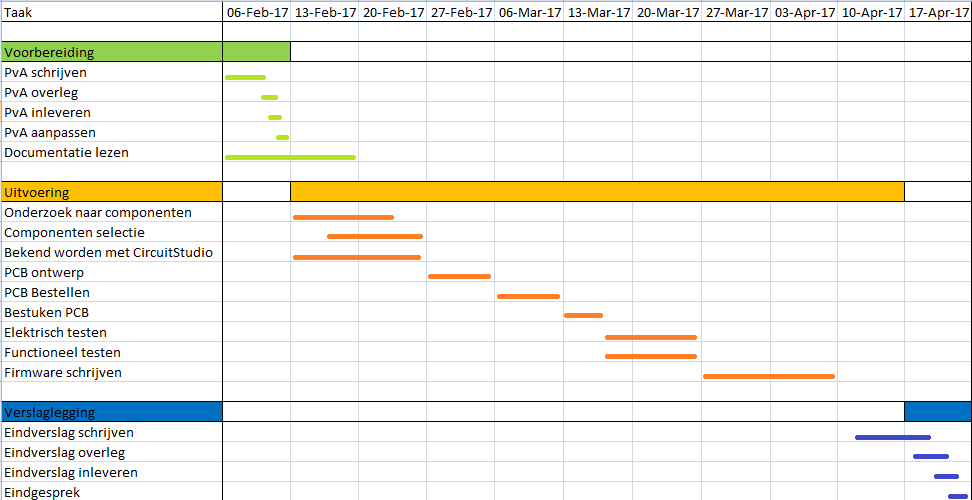
\includegraphics[width=1.0\textwidth]{figures/planning.png}
	\caption{Voorgestelde planning.}
	\label{fig:planning}
\end{figure}

Gedurende de stageperiode zijn de werktijden van 10:00 tot 17:00, voor vijf dagen in de week. Hiervan kan afgeweken worden in overleg met de stageverlener. 

\chapter{Opzet Eindverslag}
\label{ch:eindverslag}
%TODO opzet van de hoofdstukken

Het eindverslag zal in LaTEX opgemaakt worden. Daarnaast is er een geheimshoudingplicht getekend. Dit houdt in dat de begeleidende docent, ter beoordeling een volledig verslag krijgt. Voor archivering worden er passages onleesbaar gemaakt. 

\begin{enumerate}
	\item Voorblad
	\item Abstract
	\item Introductie
	\item Werkwijze/Uitvoering
	\item Resultaten
	\item Discussie
	\item Aanbevelingen
	\item Bibliografie
	\item Appendix
\end{enumerate}

\chapter{Persoonlijke Leerdoelen}
\label{ch:leerdoelen}
\section{Persoonlijke leerdoelen}
Gedurende de eerste stage zou ik vooral willen leren hoe het er aan toe gaat in een bedrijf. Mijn interesse ligt dan voornamelijk in hoe projecten gemanaged worden en hoe er omgegaan wordt met strakke deadlines. Daarnaast moeten er ook aan competenties gewerkt worden, om die naar een hoger niveau te tillen.

\section{Competenties}
In de opleiding Elektrotechniek moeten er competenties verworven worden zoals die gedefinieërd zijn in Appendix \ref{app:competenties}. 
\newline
Het doel van dit project is om een werkende PCB af te leren, en te integreren in de huidige systeem. Hierbij worden aan een aantal competenties gewerkt zoals: analyseren, ontwerpen, realiseren, onderzoeken en professionaliseren. In dit project zal er met name aandacht besteeds worden aan realiseren en professionaliseren. 
\newline
De competentie realiseren zal vooral voorkomen tijdens de productiefase van de opdracht. Hier zullen keuzes worden gemaakt over de methoden om de PCB te ontwerpen, produceren, bestuken en te testen. Binnen dit project is het belangrijk dat het makkelijk en goedkoop schaalbaar wordt. De productiemethode is dus zeer belangrijk. Daarnaast betekent ook dat alles goed gedocumenteerd moet zijn. 
\newline
Professionaliseren sluit voornamelijk aan bij mijn persoonlijke leerdoelen. Hoe worden besluiten genomen, hoe wordt er omgegaan met feedback, en hoe wordt er gecommuniceerd. Een groot gedeelte hiervan is al het strak op papier krijgen van de exacte specificicaties en wensen en verwachtingen van de stageverlener. 

\begin{thebibliography}{9}
\input{bibliography}

\end{thebibliography}

\begin{appendix}
\chapter{Stagehandleiding}
\label{app:handleiding}

\includepdf[pages={12-14}]{docs/stagehandleiding.pdf}

\end{appendix}


\end{document}
